\documentclass[11pt]{article}
\usepackage{geometry}
\usepackage{graphicx}
\usepackage{enumitem}
\usepackage{float}
\usepackage{amsmath}
\usepackage{multicol}
\usepackage{cancel}
\usepackage{mathrsfs}

\geometry{a4paper, top=0.5in, bottom=0.5in, right=0.75in, left=0.75in}

\title{Lecture 7}
\author{}
\date{}

\begin{document}

\maketitle

\section{Fabry Perot Amplifier}
It is similar to FP LASER, but we adjust the mirrors' reflectivity to prevent oscillations, so we can consider it an amplifier with a positive feedback loop but $A \beta < 1$.

\begin{center}
    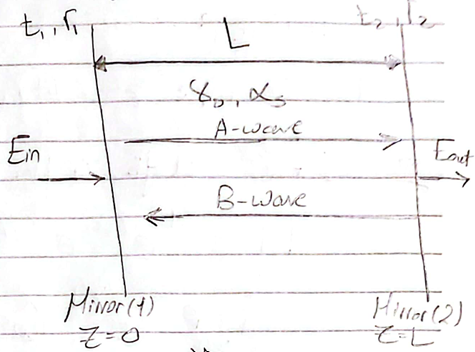
\includegraphics[scale=0.9]{1.png}
\end{center}
\begin{align}
    A(L) &= A(0) e^{-j \beta L} e^{-\frac{\alpha_s}{2} L} e^{\frac{\gamma_o}{2} L} \\
    B(0) &= B(L) e^{-j \beta L} e^{-\frac{\alpha_s}{2} L} e^{\frac{\gamma_o}{2} L} \\
    A(0) &= t_1 E_{in} + r_1 B(0) \\
    B(L) &= r_2 A(L)
\end{align}
From (3):
\begin{align}
    E_{in} = \frac{A(0) - r_1 B(0)}{t_1}
\end{align}
From (1):
\begin{align}
    E_{out} = t_2 A(L) = t_2 A(0) e^{-j \beta L} e^{-\frac{\alpha_s}{2} L} e^{\frac{\gamma_o}{2} L}
\end{align}
Substitute (4) in (2):
\begin{align}
    B(0) = r_2 A(0) e^{-2j \beta L} e^{-\alpha_s L} e^{\gamma_o L}
\end{align}
From (5) and (6):
\begin{align*}
    \frac{E_{out}}{E_{in}} &= \frac{t_1 t_2 A(0) e^{-j \beta L} e^{-\frac{\alpha_s}{2} L} e^{\frac{\gamma_o}{2} L}}{A(0) - r_1 B(0)}
\end{align*}
From (7):
\begin{align*}
    \frac{E_{out}}{E_{in}} &= \frac{t_1 t_2 e^{-j \beta L} e^{-\frac{\alpha_s}{2} L} e^{\frac{\gamma_o}{2} L}}{1 - r_1 r_2 e^{-2j \beta L} e^{-\alpha_s L} e^{\gamma_o L}}
\end{align*}

\begin{align*}
    \text{Gain} &= \frac{P_{out}}{P_{in}} = \frac{|E_{out}|^2}{|E_{in}|^2} = \frac{E_{out} E_{out}^*}{E_{in}E_{in}^*} \\
    &= \frac{t_1 t_2 e^{-j \beta L} e^{-\frac{\alpha_s}{2} L} e^{\frac{\gamma_o}{2} L}}{1 - r_1 r_2 e^{-2j \beta L} e^{-\alpha_s L} e^{\gamma_o L}} \frac{t_1^* t_2^* e^{+j \beta L} e^{-\frac{\alpha_s}{2} L} e^{\frac{\gamma_o}{2} L}}{1 - r_1^* r_2^* e^{+2j \beta L} e^{-\alpha_s L} e^{\gamma_o L}} \\
    &= \frac{|t_1|^2 |t_2|^2 e^{-\alpha_s L} e^{\gamma_o L}}{1 - 2 \Re\{r_1 r_2 e^{-\alpha_s L} e^{\gamma_o L} e^{-2j \beta L}\} + |r_1 r_2|^2 e^{-2 \alpha_s L} e^{2 \gamma_o L}}
\end{align*}
Note that $z + z^* = a + jb + a - jb = 2a = 2 \Re\{z\}$
\begin{align*}
    & \Re\{r_1 r_2 e^{-\alpha_s L} e^{\gamma_o L} e^{-2j \beta L}\} \\
    &= r_1 r_2 e^{-\alpha_s L} e^{\gamma_o L} \cos(2 \beta L) \\
    &= r_1 r_2 e^{-\alpha_s L} e^{\gamma_o L} - 2 r_1 r_2 e^{-\alpha_s L} e^{\gamma_o L} \sin^2(\beta L) 
\end{align*} 
Simplifing the denumerator:
\begin{align*}
    & 1 - 2 \Re\{r_1 r_2 e^{-\alpha_s L} e^{\gamma_o L} e^{-2j \beta L}\} + |r_1 r_2|^2 e^{-2 \alpha_s L} e^{2 \gamma_o L} \\
    &= 1 - 2 r_1 r_2 e^{-\alpha_s L} e^{\gamma_o L} + |r_1|^2 |r_2|^2 e^{-2 \alpha_s L} e^{2 \gamma_o L} + 4 r_1 r_2 e^{- \alpha_s L} e^{\gamma_o L} \sin^2(\beta L)
\end{align*}
$r_1 = \sqrt{R_1}$, $r_2 = \sqrt{R_2}$ and let $G_o = e^{-\alpha_s L} e^{\gamma_o L}$:
\begin{align*}
    \text{Gain} &= \frac{(1-R_1) (1-R_2) G_o}{1 - 2 \sqrt{R_1 R_2} G_o + R_1 R_2 G_o^2 + 4 \sqrt{R_1 R_2} G_o \sin^2(\beta L)} \\
    &= \frac{(1-R_1) (1-R_2) G_o}{(1 - \sqrt{R_1 R_2} G_o)^2 + 4 \sqrt{R_1 R_2} G_o \sin^2(\beta L)}
\end{align*}
\textbf{Notes:}
\begin{itemize}
    \item If $R_1 = R_2 = 0$ (AR coating) then Gain = $G_o$ = TWA gain
    \item If $\gamma_o = 0 \Rightarrow$ passive cavity, but if $\gamma_o \neq 0 \Rightarrow$ active cavity
    \item Note that FPA has a high gain because the waves stay in the gain medium from the mirrors reflectivity unlike the TWA where the waves leave the gain medium after the first pass.
    \item For a certain gain FPA length is less than TWA length.
    \item $G_o$ is the single path gain and more accurately is given by: $G_o = e^{-\alpha_s L} e^{\Gamma \gamma_o L}$ where $\Gamma$ is the confinement factor because the gain is only in the core (I) in the PIN structure.
\end{itemize}
\begin{center}
    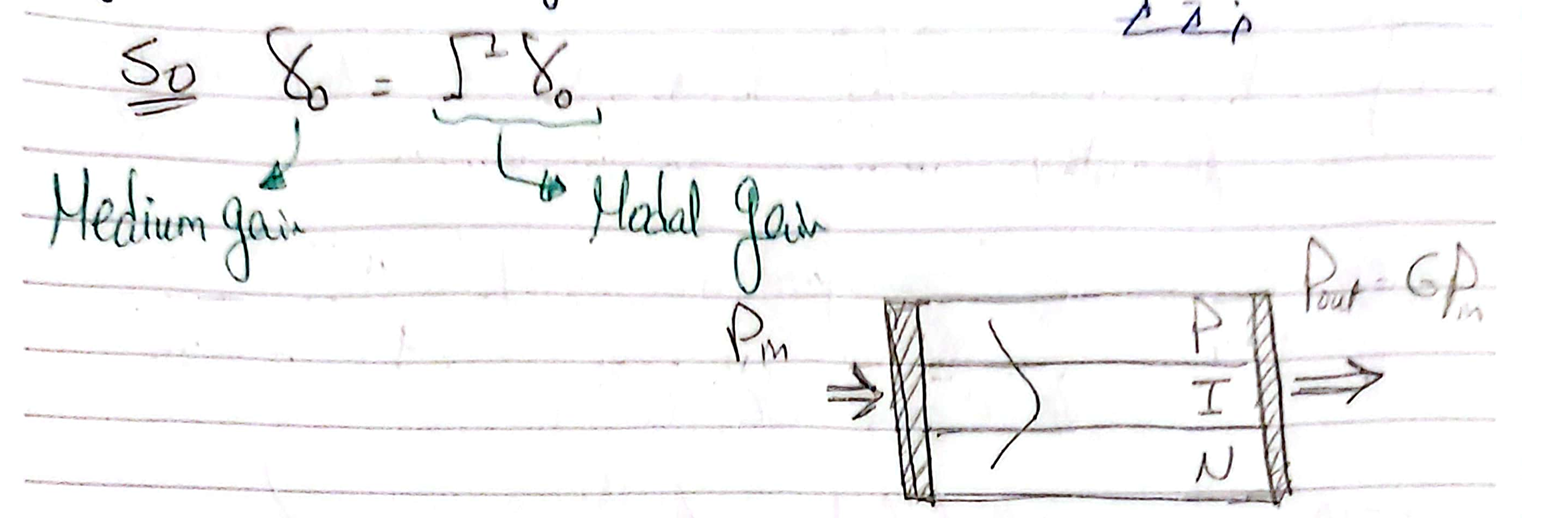
\includegraphics[scale=0.4]{2.png}
\end{center}
Maximum gain is when $\sin^2(\beta L) = 0$:
\begin{align*}
    \beta L = q \pi \rightarrow \frac{2 \pi \nu n}{c_o} L = q \pi \Rightarrow \nu_{q_{max}} = \frac{q c_o}{2 n L} = q \nu_F 
\end{align*}
where $\nu_{q_{max}}$ are the frequencies that give maximum gain and $\nu_F$ is the free spectral range ($\Delta f$ between 2 longitudinal modes in the cavity).
\begin{align*}
    Gain_{max} = \frac{(1-R_1) (1-R_2) G_o}{(1 - \sqrt{R_1 R_2} G_o)^2}
\end{align*}
Minimum gain is when $\sin^2(\beta L) = 1 \rightarrow \sin(\beta L) = \pm 1$:
\begin{align*}
    \beta L = \left(2q + 1\right) \frac{\pi}{2} \rightarrow \frac{2 \pi \nu n}{c_o} L = \left(2q + 1\right) \frac{\pi}{2} \Rightarrow \nu_{q_{min}} = \frac{\left(2q + 1\right) c_o}{4 n L}
\end{align*}
where $\nu_{q_{min}}$ are the frequencies that give minimum gain.
\begin{align*}
    Gain_{min} &= \frac{(1-R_1) (1-R_2) G_o}{(1 + \sqrt{R_1 R_2} G_o)^2 + 4 \sqrt{R_1 R_2} G_o} \\
    &= \frac{(1-R_1) (1-R_2) G_o}{1 + R_1 R_2 G_o^2 - 2 \sqrt{R_1 R_2} G_o + 4 \sqrt{R_1 R_2} G_o} \\
    &= \frac{(1-R_1) (1-R_2) G_o}{1 + R_1 R_2 G_o^2 + 2 \sqrt{R_1 R_2} G_o} \\
    &= \frac{(1-R_1) (1-R_2) G_o}{(1 + \sqrt{R_1 R_2} G_o)^2}
\end{align*}
Note that $G_o$ is frequency dependent because $\gamma_o$ is frequency dependent, so the gain is frequency dependent.
\begin{center}
    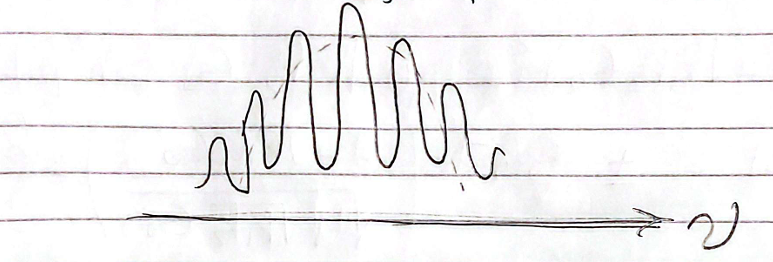
\includegraphics[scale=0.8]{3.png}
\end{center}
We will define a new parameter called the ripples $\rho = \frac{G_{max}}{G_{min}}$. This parameter puts a spec on the AR coating reflectivity when designing a TWA.
\begin{align*}
    \rho_{dB} = 10 \log \left(\frac{G_{max}}{G_{min}}\right) = 20 \log \left(\frac{1 + \sqrt{R_1 R_2 G_o}}{1 - \sqrt{R_1 R_2 G_o}}\right)
\end{align*}
To get FWHM:
\begin{align*}
    G \left(\nu + \frac{\Delta \nu}{2}\right) = \frac{G_{max}}{2} = \frac{(1-R_1) (1-R_2) G_o}{2(1 - \sqrt{R_1 R_2} G_o)^2} = \frac{(1-R_1) (1-R_2) G_o}{(1 - \sqrt{R_1 R_2} G_o)^2 + 4 \sqrt{R_1 R_2} G_o \sin^2(\beta L)}
\end{align*}
So:
\begin{align*}
    & (1 - \sqrt{R_1 R_2} G_o)^2 = 4 \sqrt{R_1 R_2} G_o \sin^2(\beta L) \\
    & \beta L = \pm \sin^{-1}\left(\frac{1 - \sqrt{R_1 R_2} G_o}{\sqrt{4 \sqrt{R_1 R_2} G_o}} \right) = \frac{2 \pi \nu_{1,2} n}{c_o}L \\
\end{align*}
So:
\begin{align*}
    \Delta \nu_{FWHM} = \nu_1 - \nu_2 = 2 \frac{c_o}{2 \pi n L} \sin^{-1}\left(\frac{1 - \sqrt{R_1 R_2} G_o}{\sqrt{4 \sqrt{R_1 R_2} G_o}} \right)
\end{align*}
\begin{center}
    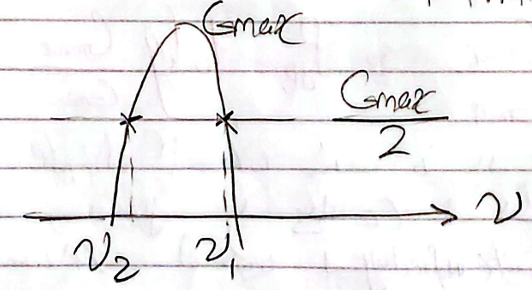
\includegraphics[scale=0.8]{4.png}
\end{center}
$\frac{c_o}{\pi n L} = \frac{c_o}{2 n L} \frac{2}{\pi} = \nu_F \frac{2}{\pi}$, so:
\begin{align*}
    \Delta \nu_{FWHM} = \frac{2}{\pi} \nu_F \sin^{-1}\left(\frac{1 - \sqrt{R_1 R_2} G_o}{\sqrt{4 \sqrt{R_1 R_2} G_o}} \right)
\end{align*}
$\sin^{-1}(x) \approx x$ if $x << 1$, so if $G_o >> 1$ and $R = \sqrt{R_1 R_2}$:
\begin{align*}
    \Delta \nu_{FWHM} \approx \frac{2 \nu_F}{\pi}  \frac{1 - \sqrt{R_1 R_2} G_o}{\sqrt{4 \sqrt{R_1 R_2} G_o}} = \frac{\nu_F}{\pi} \frac{1 - R G_o}{\sqrt{R} G_o}
\end{align*}
We will define a new parameter Finesse (F), which is similar to the Quality factor ($Q = \frac{f}{\Delta f}$). Q is used when having a single resonnance frequency, but F is used when having multiple resonnance frequencies. Higher F means better selectivity.
\begin{align*}
    F = \frac{\nu_F}{\Delta \nu} = \frac{\pi \sqrt{R} G_o}{1 - R G_o}
\end{align*}
Finesse is usually defined for a passive cavity (such as an ideal filter), where there is no loss or gain ($\gamma_o = \alpha_s = 0$, so $G_o = 1$):
\begin{align*}
    F = \frac{\pi \sqrt{R}}{1 - R}
\end{align*}
In case of a practical filter, $\gamma_o = 0$ and $\alpha_s \neq 0$, so $G_o = e^{-\alpha_s L}$:
\begin{align*}
    F = \frac{\pi \sqrt{R} e^{-\alpha_s L}}{1 - R e^{-\alpha_s L}}
\end{align*}
Another equation for practical filter Finesse is:
\begin{align*}
    & \alpha_r = \alpha_s + \frac{1}{2L} ln\left(\frac{1}{R_1 R_2}\right) = \alpha_s + \frac{1}{L} ln\left(\frac{1}{\sqrt{R_1 R_2}}\right) = \alpha_s + \frac{1}{L} ln\left(\frac{1}{R}\right) \\
    & e^{-\alpha_r L} = e^{-\alpha_s L} e^{-ln\left(\frac{1}{R}\right)} = e^{-\alpha_s L} e^{ln(R)} = R e^{-\alpha_s L} \\
    & F = \frac{\pi \sqrt{R} e^{-\frac{\alpha_s}{2} L}}{1 - R e^{-\alpha_s L}} = \frac{\pi e^{-\frac{\alpha_r}{2} L}}{1 - e^{-\alpha_r L}}
\end{align*}
If $\alpha_r L << 1$ then $1 - e^{-\alpha_r L} \approx \alpha_r L$, so:
\begin{align*}
    F = \frac{\pi (1 - e^{-\frac{\alpha_r}{2} L})}{\alpha_r L} = \frac{\pi}{\alpha_r L} 
\end{align*}
FPA is FP LASER if gain tends to infinity, so $G_{max} \rightarrow \infty$:
\begin{align*}
    1 - \sqrt{R_1 R_2} G_o = 0 \Rightarrow G_o = \frac{1}{\sqrt{R_1 R_2}}
\end{align*}
Using $G_o = e^{-\alpha_s L} e^{\gamma_o L}$:
\begin{align*}
    & e^{-\alpha_s L} e^{\gamma_o L} = \frac{1}{\sqrt{R_1 R_2}} \Rightarrow (\gamma_o - \alpha_s)L = \frac{1}{2} ln\left(\frac{1}{R_1 R_2}\right) \\
    & \Rightarrow \gamma_o = \alpha_s + \frac{1}{2L} ln\left(\frac{1}{R_1 R_2}\right) 
\end{align*}
Photon lifetime is the time a photon stays in the cavity before leaving it, which controls the bandwidth of the cavity. The photon lifetime is given by:
\begin{align*}
    \tau_{ph} = \frac{1}{\alpha_r v_g} \approx \frac{n}{\alpha_r c_o} 
\end{align*}
Proof:
\begin{align*}
    I(z) &= I(0) e^{-\alpha_r z} \\
    \frac{dI(z)}{dz} &= -\alpha_r I(0) e^{-\alpha_r z} = -\alpha_r I(z)
\end{align*}
So:
\begin{align*}
    \frac{dI}{dt} = \frac{dI}{dz} \frac{dz}{dt} = -\alpha_r I v_g = -\alpha_r I \frac{c_o}{n}
\end{align*}
So:
\begin{align*}
    I(t) = I(0) e^{-\alpha_r \frac{c_o}{n} t} \Rightarrow \tau_{ph} = \frac{1}{\alpha_r c}
\end{align*}
If losses decrease, the photon lifetime increases meaning it will stay longer in the cavity. 

\end{document}